\documentclass[openany,12pt]{report}

\setlength{\textwidth}{6.25in} % original 6.25

\setlength{\textheight}{8.9in}

\renewcommand{\baselinestretch}{1.3}

%\headheight 12.0pt

\oddsidemargin 20pt    %  Left margin on odd-numbered pages.

\evensidemargin 20pt   %  Note that \oddsidemargin = \evensidemargin

\topmargin 0pt

%\headsep 10pt

\footskip 10.0pt

\usepackage {graphics}

\usepackage[colorinlistoftodos]{todonotes}

\usepackage{comment}

%\usepackage {algorithm}

%\usepackage {algorithmic}
\usepackage{hyperref}
\usepackage{color}
\usepackage{lastpage} % for the number of the last page in the document
\usepackage{fancyheadings}
\pagestyle{fancy}
\usepackage {epsfig}
\usepackage {graphicx}
\usepackage{float}
\usepackage{array} % for making text bold in table
\usepackage{longtable}
%\usepackage[dvips, bookmarks, colorlinks=false]{hyperref}
%\usepackage{hyperref} %for creating links in the pdf version and other additional pdf attributes, no effect on the printed document

%*****************************Title Page**************************************************************

\begin{document} % Begin document "environment".
	\lhead{}
	\chead{}
	\rhead{Artificially Intelligent Traffic Management System}
	\lfoot{ MET's Institute of Engineering}
	\setlength{\headrulewidth}{0.4pt}
	\setlength{\footrulewidth}{0.4pt}
	\fontsize{12}{15}
	\begin{titlepage}
		\begin{center}
			%\vspace{0.2in}
			{\bf A Project Report on} \\
			\vspace{0.3in}
			{\Large \bf ``Artificially Intelligent Traffic Management System''}\\
			\vspace{0.3in}
			SUBMITTED TO THE SAVITRIBAI PHULE UNIVERSITY, PUNE\\
			IN THE PARTIAL FULFILMENT OF THE REQUIREMENTS \\
			FOR THE AWARD OF THE DEGREE \\
			\vspace{0.2in}
			OF\\  
			\vspace{0.2in}
			BACHELOR OF ENGINEERING (COMPUTER ENGINEERING)\\
			(Academic Year: 2021-22)\\
			\vspace{0.2in}
			
			{\it SUBMITTED BY}\\
			
			\vspace{0.2in}
			
			{\bf Mr. Saquib Akhtar Aneesur Rahman}\hspace*{\fill}{\bf (Div - B Roll No. 03)}\\
			{\bf Mr. Giwil Gidwani }\hspace*{\fill}{\bf (Div - A Roll No. 24)}\\
			{\bf Mr. Vrushabh Nikam Dattatray     }\hspace*{\fill}{\bf (Div - B Roll No. 50)}\\
			{\bf Mr. Rutuja Rajesh Shinde    }\hspace*{\fill}{\bf (Div - B Roll No. 46)}\\
			
			\vspace{0.4in}
			
			{\it Under the guidance of}\\
			
			\vspace{0.1in}
			
			{\bf Mr. Ravindra Aher}\\
			\vspace{0.4in}
			
			
			{\small DEPARTMENT OF COMPUTER ENGINEERING}\\
			\begin{figure*}[h]
				\centerline{\psfig{figure=./metbkc.eps,width=4.1in,height=0.5in}}
				\label{atcres}
			\end{figure*}
			{\large MET's Institute of Engineering,}\\
			{\small Adgaon, Nashik-422003}\\
			SAVITRIBAI PHULE UNIVERSITY, PUNE\\
			\vspace{0.2in}
			{\small December, 2021}
		\end{center}
	\end{titlepage}
	
	%*****************************Certificate*************************************************************
	\fontsize{14}{16}
	\thispagestyle{empty}
	\begin{center}
		\begin{figure*}[h]
			\centerline{\psfig{figure=./metbkc.eps,width=7.2in,height=1.2in}}
			\label{atcres}
		\end{figure*}
		\vspace{0.1in}
		{\it \Huge  \textbf{Certificate}}
		\vspace{0.2in}\\
		{\it This is to Certify that the project report entitles}\\
		\vspace{0.2in}
		{\Large \bf ``Artificially Intelligent Traffic Management System''}\\
		\vspace{0.2in}
		
		{\bf Mr. Saquib Akhtar Aneesur Rahman}\hspace*{\fill}{\bf (Seat No.\hspace*{1.5in})}\\
		{\bf Mr. Giwil Gidwani  }\hspace*{\fill}{\bf (Seat No.\hspace*{1.5in})}\\
		{\bf Mr. Vrushabh Nikam Dattatray     }\hspace*{\fill}{\bf (Seat No.\hspace*{1.5in})}\\
		{\bf Ms. Rutuja Rajesh Shinde    }\hspace*{\fill}{\bf (Seat No.\hspace*{1.5in})}\\
	\end{center}
	\vspace{0.3in}
	{\it are bonafide students of this institute and the work has been carried out by them under
		the guidance of Mr. Ravindra Aher and it is approved for the partial fulfillment of the
		requirement of Savitribai Phule Pune University for the award of the degree of Bachelor
		of Engineering (Computer Engineering).}\\
	\vspace{0.2in}
	\vspace{0.7in}
	\noindent
	
	\hspace{0.1in} Project Guide  \hspace{1.5in}H.O.D \hspace{0.9in} Principal  \\
	\hspace{4.6in} (Mr. Ravindra Aher) \hspace{0.6in}(Dr. M. U. Kharat)\hspace{0.4in}(Dr. V. P. Wani)\\
	\vspace{0.2in}
	
	Date: \hspace{0.2 in}/\hspace{0.3 in}/   \\
	\newpage \pagenumbering{Roman}
	%\vskip
	\chapter*{Acknowledgements}
	
	\hspace*{0.5 in}We have taken efforts in this project. However, it would not have been possible without the kind support and help of many individual and organizations. We would like to extend our sincere thanks to all of them. It gives us proud privilege to complete the project on \textbf{ ``Artificially Intelligent Traffic Management System''}. We are highly indebted to our internal guide \textbf{Mr. Ravindra Aher} for his guidance and constant supervision as well as for providing necessary information regarding the project and also for his support in completing the project.\\
	
	\hspace*{0.5 in}We are also extremely grateful to our respected H.O.D. (Computer Department) \textbf{Dr. M. U. Kharat} and \textbf{Prof. Dr. Priti Metange} (Project Co-ordinator) for providing all facilities and every help for smooth progress of project work.\\
	\\
	\hspace*{3.5 in}Mr. Saquib Akhtar Aneesur Rahman\\
	\hspace*{3.5 in}Mr. Giwil Gidwani \\
	\hspace*{3.5 in}Mr. Vrushabh Nikam Dattatray\\
	\hspace*{3.5 in}Ms. Rutuja Rajesh Shinde
	
	%*****************************Abstract*************************************************************
	\chapter*{Abstract\markboth{Abstract}{Abstract}}
	\hspace*{0.5 in}Congestion of traffic in urban areas and smart cities is one of the major issues with increasing population in metropolitan areas. Traffic jams are not only a cause of delay and inconvenience in day to day life but also a major source of noise and air pollution.
	Modern approaches to deal with this issue range from complicated software handling dozens of traffic signals throughout an entire city to simpler single-intersection solutions. However these can be costly, difficult to implement and may require a lot of manual monitoring.\\
	\\
	\hspace*{0.5in}This project proposes a traffic management system which uses concepts from artificial intelligence and graph theory to control and optimize traffic flow. Its aim is to optimize traffic flow on a small to medium scale in a manner which adapts to the real time changes in traffic.\\
	
	\newpage
	\tableofcontents
	\listoffigures
	\listoftables
	\newpage	
	\pagenumbering{arabic}
	
	
	
	
	%*****************************Chapter1 *****************************
	
	\chapter{Introduction}
	\hspace*{0.5in}This chapter briefly explains the need for an adaptive traffic management system and an overview of the implementation.\\
	
	\section{Overview}
	\hspace*{0.5in}Traffic congestion is becoming one of the critical issues in cities with increasing population and number of vehicles. They not only cause problems like delays and stress to drivers but also cause secondary problems like increasing fuel consumption, transportation costs and pollution.
	
	The causes of congestion can be divided into two categories, recurring and non recurring congestion. Recurring congestion can be expected to occur at the same time every weekday as a result of high volumes of commuter traffic traveling on roadways that are at or near their carrying capacity. Non-recurring congestion occurs as a result of an unexpected or non-typical event. Some causes of non-recurring congestion include: vehicular crashes, vehicle breakdowns, roadway construction, inclimate weather, and additional traffic resulting from special events. While non-recurring congestion can be unpredictable and difficult to treat, recurring congestion can be reduced by increasing road capacity or with the help of adaptive traffic control systems.
	
	There are several existing standardized solutions for adaptive traffic control such as SCOOT, SCAT, etc. which have been implemented in many major metropolitan cities. However, most suburban and urban areas use conventional traffic control systems such as manual traffic control or non adaptive automated traffic control. Manual control consists of an on-site traffic official guiding vehicles. Non adaptive automated traffic control refers to the use of fixed timers in traffic signals. Wide implementation of standardized adaptive traffic control is not possible due to lack of feasibility since it requires manual labor and installation of new sensors. Therefore a more feasible solution which reuses existing infrastructure is required.
	
	This project proposes an Artificially Intelligent Traffic Management System which uses existing CCTV feed and API data if needed to optimize traffic control over small to medium scale road networks. It uses an artificially intelligent agent or model to handle the complexity of day to day traffic in real-time. Furthermore, simulations will be performed to demonstrate and test the model.\\
	
	\section{Summary}
	\hspace*{0.5in}This chapter discusses the need for an intelligent traffic management system and also discussed a brief overview of the project.\\
	%*************************Chapter 2************************
	\chapter{Literature Survey}
	
	\hspace*{0.5in}This chapter consists of the various studies and research conducted on key concepts which are essential to create and understand the proposed system.
	
	\section{You Only Look Once: Unified, Real-Time Object Detection, Joseph Redmon, et al. \cite{paper1}}
	\hspace*{0.5in}Object detection comprises locating specific types of objects in an image or video. The output of a typical object detection algorithm consists of bounding box coordinates and a label of the object. YOLO (You Only Look Once) model consists of an extremely fast unified architecture for object detection. It makes use of a single neural network for predicting bounding boxes and class probabilities from a full image in a single evaluation. Hence, making it ideal for object detection in real time applications.\\
	
	\section{Traffic Congestion Detection from Camera Images using Deep Convolution Neural Networks, Pranamesh Chakraborty, et al. \cite{paper2}}
	\hspace*{0.5in}Recent improvements in computer vision algorithms have led to closed-circuit television (CCTV) cameras emerging as an important data source for determining the state of traffic congestion. To detect congestion in a traffic CCTV footage YOLO, a state-of-the-art real-time object detection algorithm is used. In the above mentioned paper, several object detection techniques were tested for congestion detection out of which YOLO showed the most promising results.\\
	
	\section{Smart Control of Traffic Light Using Artificial Intelligence, Mihir M. Gandhi, et al. \cite{paper3}}
	\hspace*{0.5in}Traffic signal timing plays an important role in controlling flow and efficiency of traffic.
	The above system makes use of vehicle count obtained from CCTV footage and uses it to  optimize green signal timing for each lane to optimize traffic flow at a single intersection. The aim of the project is to create a similar system and extend the scope of optimization to multiple adjacent intersections.\\
	
	\section{Comparison of Current Practical Adaptive Traffic Control Systems, Hongyun Chen, et al. \cite{paper4}}
	\hspace*{0.5in}Existing Adaptive Traffic Control Systems (ACTS) such as SCOOT, SCAT, OPAC, RHODES, etc. are being adapted by major cities in developed and developing countries. They can cover up to hundreds (OPAC) to even thousands (SCOOT, SCAT) of intersections. However, their implementation includes installation of additional sensors and can lead to very heavy costs which isn't feasible for smaller cities. Additionally, these systems do not take into consideration challenges such as power failure, non lane following traffic and mixed traffic which are common in Indian roads.\\
	\hspace*{0.5in}The aforementioned systems provide key algorithmic insights for developing a more feasible ACTS model. Furthermore, usage of existing inputs such as CCTV needs to be emphasized over installation of new sensors in order to help reduce costs.\\
	
	\section{Summary}
	\hspace*{0.5in}This chapter reviews research done on key concepts such as object detection and implementation of artificial intelligence with traffic signals which are essential to the proposed system. Existing solutions, their inner workings as well as their advantages and disadvantages were studied.\\
	
	
	%*************************Chapter 3 ************************
	
	\chapter{Problem Definition}
	
	\hspace*{0.5in}This chapter discusses the drawbacks of current systems implemented in suburban and urban areas and also defines the need and overall scope of an artificially intelligent traffic management system.\\
	
	\section{Need For Artificially Intelligent Traffic Management Systems}
	\hspace*{0.5in}Traffic congestion is becoming a critical issue with increasing population and automobiles in cities. The conventional systems which were suitable at the time of their installation may not be suitable in the present time due to the rising number of vehicles. Furthermore, upgrading these systems to the standards used in major metropolitan cities is often not feasible due to several factors such as manual labor and installation of new sensors. Owing to these factors, the majority of intersections make use of either manual control which includes traffic police officials guiding vehicles or non adaptive automatic control, which includes the use of fixed timers. In most scenarios these solutions may not be at par with the unpredictable rate of traffic flow. Hence, an intelligent, adaptive and feasible solution is needed.\\
	
	\section{Additional Features}
	\hspace*{0.5in}Additionally, the following points must be kept in mind while developing or optimizing an automated traffic controlling system:\\
	
	\begin{itemize}
		\item{Ensuring necessary fall backs in case of disconnection or power cuts.}
		\item{Ensuring signal times are between a maximum and minimum limit to avoid starvation.}
		\item{Indian traffic is not lane following and has a high amount of mixed traffic. System must be able to withstand these challenges.}
		\item{The system must make use of existing sensors and avoid installation of newer sensors in order to maintain feasibility.}
		\item{The system must be scalable within budget and it should be able to handle an increasing number of vehicles.}
		\item{Additional features such as incident detection, report generation and assistance for emergency or VIP vehicles are desirable.}
	\end{itemize}
	
	
	
	\section{Summary}
	\hspace*{0.5in}This chapter discusses the need of artificially intelligent traffic management systems and the various points which must be kept in mind while developing said system.\\
	
	%*****************************Chapter 4******************
	
	\chapter{Analysis}
	\begin{comment}
		\hspace*{0.5in}This chapter describes the project plan adopted and determines the requirement analysis. We have implemented the project on the basis of Rapid Application Development (RAD) model and Model View Controller (MVC) model. The stake holders who participated in the requirement analysis process were the developers of Cognifront who will be among the end users of the Artificially Intelligent Traffic Management System for building M- Applications.
	\end{comment}
	
	\hspace*{0.5 in}This chapter describes the project plan adopted and determines the requirement analysis. The project was implemented on the basis of Agile model and Model View view-model.
	
	
	\section{Project Plan}
	
	\subsection{Project Plan for semester I}
	
	\hspace*{0.5 in}The following Table 4.1 describes the project plan for semester I. It describes the various activities and accountability of the developers for the respective modules. Following are the major activities carried out in this plan :
	\begin{itemize}
		\item{Identifying the functional requirements.}
		\item{Designing of the Framework.}
		\item{Studying the necessary development tools and technologies.}
	\end{itemize}
	
	\newpage
	\begin{table} [htb]
		\centering
		\begin{tabular}{| p{1.2 cm}| p{5 cm}| p{2.5 cm}| p{2.5 cm}| p{3 cm}| }\hline
			\textbf{Phase}	&\textbf{Activity}	&\textbf{Start Date}	&\textbf{End Date} &\textbf{Group Members}\\\hline\hline
			1 &Selection of Project Topic	&22-08-2021 	&25-08-2021 &Team \\\hline
			1 &Functional Requirement Specification(FRS) &29-08-2021 &09-09-2021 &Team\\\hline
			1 &Design Prototype &11-09-2021 &21-09-2021 &Team\\\hline
			1 &Set Theory and Math Model &23-09-2021 &06-10-2021 & Saquib, Giwil\\\hline
			1 &UML Diagram Prototype &23-09-2021 &03-10-2021 &Vrushabh, \newline Rutuja \\\hline
			1 &Project Problem Statement using NP Complete &08-10-2021 &19-10-2021 &Saquib, Giwil\\\hline
			1 &UML Diagram in StarUML &05-10-2021 &22-10-2021 &Team \\\hline
			1 &Paper Presentation &05-11-2021 &05-11-2021 &Team \\\hline
			1 &Software Requirement Specification &6-11-2021 &10-11-2021 &Team \\\hline
			1 &Test Plan &11-11-2021 &15-11-2021 &Vrushabh, \newline Rutuja \\\hline
		\end{tabular}
		\caption{Planner and Progress Report I for AITMS}
		\label{tab:nnwork}
	\end{table}

	\begin{comment}
		\hspace*{0.5 in}The following Table 4.2 describes the project plan for semester II. It describes the various activities and accountability of the developers for the respective modules. Following are the major activities carried out in this plan :
		\begin{itemize}
			\item{Define Programming Standards.}
			\item{Development of project in 3 Milestones.}
			\item{Formal Technical Review and Testing.}
		\end{itemize}
		\newpage
		\begin{table} [htb]
			%\centering
			\begin{tabular}{| p{1.2 cm}| p{5 cm}| p{2.5 cm}| p{2.5 cm}| p{3 cm}| }\hline
				\textbf{Phase}	&\textbf{Activity}	&\textbf{Start Date}	&\textbf{End Date} &\textbf{Group Members}\\\hline\hline
				2 &Defining Programming Standards	&10-12-2021 	&15-12-2021 &Team \\\hline
				2 &Development of Milestone No.1 &16-12-2021 &05-01-2012 &Team\\\hline
				2 &Development of Milestone No.2 &7-01-2012 &02-02-2012 &Team\\\hline
				2 &Development of Milestone No.3 &05-02-2012 &29-02-2012 & Team \\\hline
				2 &Formal Technical Review &02-03-2012 &10-03-2012 &Team \\\hline
				2 &Testing and Bug Fixing  &22-03-2012 &10-04-2012 &Team\\\hline
				
			\end{tabular}
			\caption{Planner and Progress Report II for Maggie}
			\label{tab:nnwork}
		\end{table}
	\end{comment}
	
	
	\section{Requirement Analysis}
	
	\subsection{Necessary Functions}
	\begin{itemize}
		\item{Deliver a reusable piece of code.}
		\item{Build an application and}
		\item{Deployment of application built onto the Windows.}
	\end{itemize}
	
	\subsection{Desirable  Functions}
	\begin{itemize}
		\item{Assistance to emergency and VIP vehicles.}	
		\item{Traffic incident detection.}
		\item{Real-time Traffic Congestion Detection.}
		\item{Real-time Statistics.}
		
	\end{itemize}
	
	\section{Summary}
	\hspace*{0.5in}This chapter describes the implementation details of the project plan for Semester I. The necessary functions and the desirable functions of Artificially Intelligent Traffic Management System were also studied.
	%*****************************Chapter5***************
	\chapter{Design}
	\hspace*{0.5in}This chapter describes the Software Requirement Specification (SRS) to be implemented for Artificially Intelligent Traffic Management System. It also explains the architecture of the system and external interface requirements.\\
	
	\section{Software Requirement Specifications}
	\hspace*{0.5in} The Software Requirement Specification describes the scope of the project, operating environment, user characteristics, design and constraints. It also elaborates the system architecture of the Artificially Intelligent Traffic Management System.
	
	\subsection{Project Scope}
	
	\hspace*{0.5in}The main purpose of developing the Artificially Intelligent Traffic Management System is for the welfare of the public and reduce the pollution caused by traffic congestion. The issue of transportation is one of the most problematic issues in the country, and in the world at large. In an age where a person has a private car, and especially in countries where there is a failing public transport system, traffic jams and the countless accidents that accompany road congestion harm the economic, political aspect and social in both the public and private sectors. the transportation systems used by transportation agencies around the world are not adapted to modern transportation - these are systems designed decades ago, when the amount of cars on the roads was much smaller than today, and the transportation nodes were relatively simple. today, innovative technologies for computerized transportation management are in use, but these turned out to be extremely expensive, and due to budget shortages and even many cuts in the transportation budget, transportation agencies are often forced to give up these systems and stick with the old systems.countries such as Australia, Singapore, and a number of U.S. states have adopted transportation management technologies on a massive scale (for example, GLIDE, SCATS - these are huge economic investments, but they are prove themselves as highly prudent and effective investments. The purpose of the software is to enable the optimization of transportation traffic through the optimization of node activity transportation, and adjusting their mode of operation in real time to the transportation traffic at any given moment. The software is intuitive and accessible as much as possible, while maintaining accuracy, maximum detail, level of performance And high efficiency.
	\\The scope of Artificially Intelligent Traffic Management System can be considered as a collection of reusable piece of code, style-sheets and include files that can be used by the developer for developing more advanced systems and also considering the following points :
	\begin{itemize}
		\item{Warehousing of parametric data and reports to analyze periodic patterns and improve optimization using it (data science)}
		\item{Making AITMS compatible with each other so that neighboring solutions can work together providing another layer of optimization with added scalability}
	\end{itemize}
	
	\subsection{Operating Environment}
	\hspace*{0.5in}The proposed system will require an operating environment with appropriate version of windows OS, python, tensorflow and sufficient computation power through GPUs.
	
	\subsection{Design and Implementation Constraints}
	\hspace*{0.5in}
	The key restriction here will be to verify the validity of the report,which is not always feasible.Security threats may be involved.\\
	\begin{itemize}
		\item{\textbf{Memory:} Minimum 16GB RAM}
		\item{\textbf{CPU:} Intel Core i5 - 8300H or equivalent\textbackslash higher.}\\
		\item{\textbf{GPU:} Nvidia GTX 1050ti or equivalent\textbackslash higher.}
		\item{\textbf{LAN for CCTV:}  CCTV feed from intersections to the server room.}
		\item{\textbf{Operating System:}  This application works on Windows.}
	\end{itemize}
	
	\subsection{Assumptions and Dependencies}
	\hspace*{0.5in}The Framework is capable of allowing the developer to develop the more advanced application for Traffic Congestion Clearance. The Admin has a
	computer with graphic card, gets to monitor intersections and rest of the system is automated.
	
	
	\newpage
	\section{System Architecture}
	
	\hspace*{0.5in}The overall architecture can be viewed in the form of a  3 layer architecture consisting of physical intersection, intersection node and the optimizer.\\
	\begin{figure}[H]
		\centering
		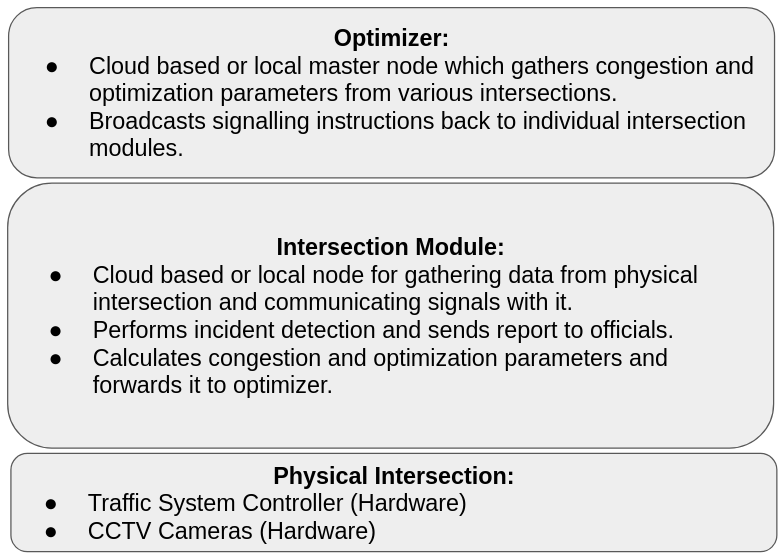
\includegraphics[width=5.2in,height=4.5in]{./Diagrams/PNG/layered_architecture}
		\caption{Layered form of System Architecture}
	\end{figure}
	
	\hspace*{0.5in}The lowermost layer i.e. the physical intersection consists of the physical traffic signal controllers and CCTV cameras. This layer contains the pre-existing infrastructure used for controlling traffic. The traffic signal controller must provide an interface to obtain and control its state. Furthermore, real-time CCTV footage must be made available to the model.\\
	
	\hspace*{0.5in}The intermediate layer consists of intersection nodes (software). Each intersection node represents a single traffic intersection. Intersection nodes serve the following primary functions:\\
	
	\begin{itemize}
		\item{Collecting CCTV footage and other data from physical intersection layer and APIs (if required by optimizer).}
		\item{Obtaining optimizer parameters from the collected raw data. For example, obtaining vehicle count from CCTV footage using YOLO. The intersection node then forwards this data to the optimizer.}
		\item{Intersection nodes also receive timing signals as outputs from the optimizer, their task is to then interface these signals onto the controller.}
	\end{itemize}
	
	\hspace*{0.5in}Aside from the above functions, the intersection nodes can also be used to perform extra tasks such as incident detection and sending reports on traffic incidents and congestion to traffic officials. It must be noted that since intersection nodes are services in execution, they can be executed over cloud or locally depending on feasibility. Depending on availability of computation power and hardware setup, a single computing device can hold multiple intersection nodes as well.\\
	
	\hspace*{0.5in}The uppermost layer consists of the optimizer. The optimizer is the master node which receives the required data from all the intersection nodes and executes the optimization algorithm. The optimization algorithm gives the signal timing details as output in terms of green signal time which is broadcasted back to the respective intersection nodes.\\
	
	\hspace*{0.5in}Several optimization algorithms were selected which can be applied depending on their performances on a simulation consisting of a specific map. It should also be noted that different optimization algorithms may be suited for different maps.\\
	
	\begin{figure}[H]
		\centering
		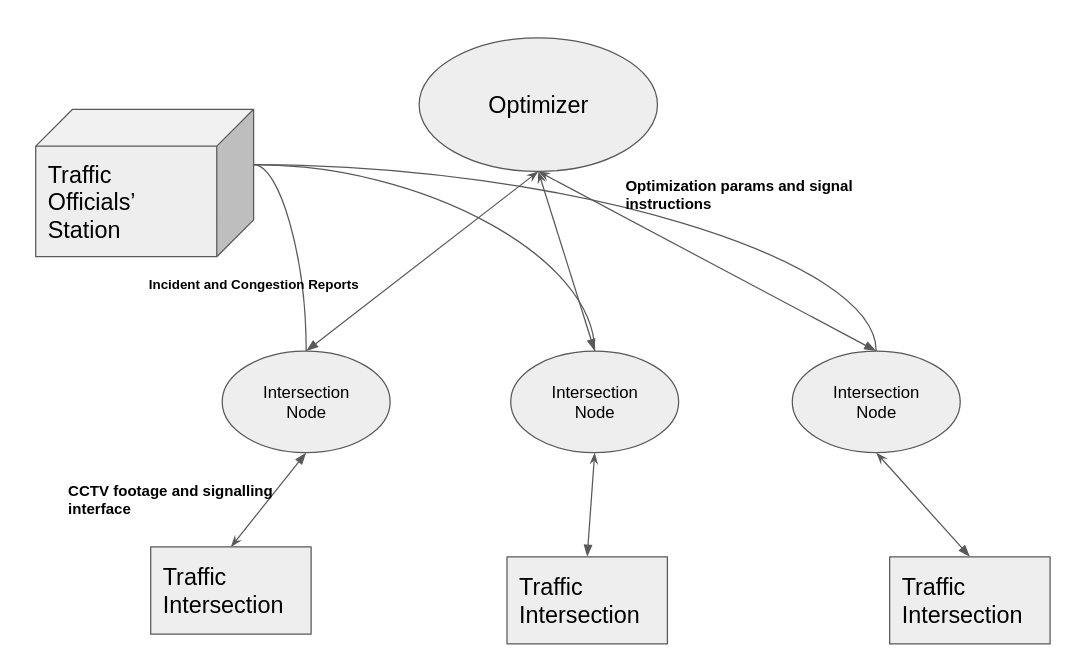
\includegraphics[width=6.5in,height=5.5in]{./Diagrams/PNG/architecture}
		\caption{System Architecture Illustration}
	\end{figure}
	
	\begin{comment}
		content...
		
		\section{External Interface Requirement}
		
		\subsection{User Interfaces}
		
		\begin{itemize}
			\item{\textbf{Desktop Application:}  Using the desktop application the end user will be able to provide the M-Learning content for the application to be developed using the Artificially Intelligent Traffic Management System.}
			\item{\textbf{M-Learning Application:}  The M-Learning application will provide a Graphical User Interface which will consist of several screens which the end user will be able to navigate to consume learning.}
		\end{itemize}
		
		\subsection{Hardware Interfaces}
		\begin{itemize}
			\item{\textbf{Mobile Devices:} The M-Learning applications built using the framewok will be deployed on mobile devices like smart-phones and tablets supporting Android operating system version 2.2 and above.}
			\item{\textbf{SD card:}  The M-Learning application will load the learning content stored on the SD card. End user will be able to write on the SD card as well.}
		\end{itemize}
		
		\subsection{Communication Interfaces}
		\hspace*{0.5in}The M-Learning application will be communicating through the internet via a Transmission Control Protocol of the TCP/IP suite for Social Networking Interface(SNI) and video streaming.
		
	\end{comment}
	\section{Software System Attribute}
	\begin{itemize}
		
		\item{\textbf{Reliability:} The traffic management system should be reliable with necessary fallbacks in case of technical failuers.}
		
		\item{\textbf{Maintainability:}  The Artificially Intelligent Traffic Management System shall be well documented and easy for developers to improve on}
		
	\end{itemize}
	
	\section{Data Flow Diagram}
	
	\hspace*{0.5in}The Data Flow Diagram explains the flow of information in the project, i.e. it indicates from where data or information is received (input) and to where it is sent (output). The Data Flow Diagrams for the project are given below:\\
	
	\begin{figure}[H]
		\centering
		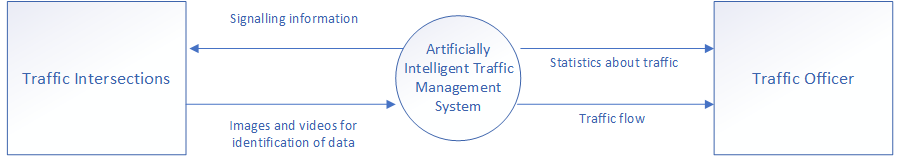
\includegraphics[width=6.8in,height=1.5in]{./Diagrams/PNG/dfd0}
		\caption{Level 0 Data Flow Diagram}
	\end{figure}
	
	\begin{figure}[H]
		\centering
		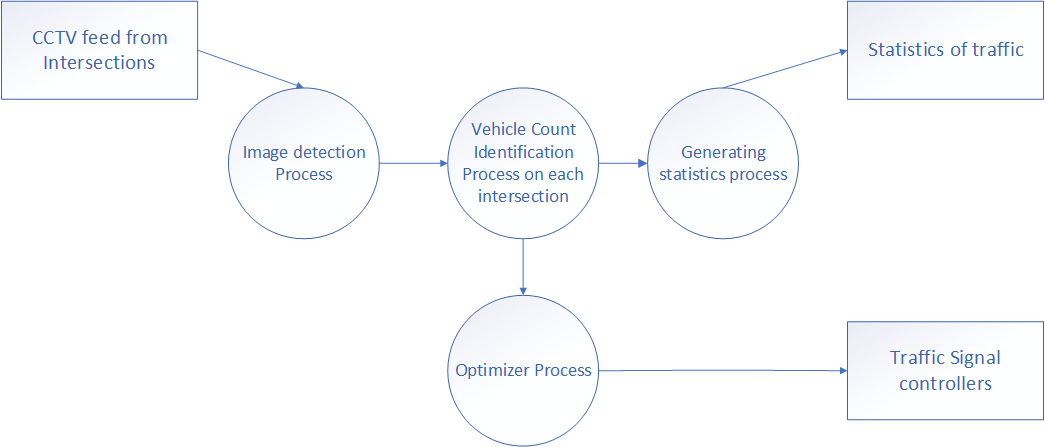
\includegraphics[width=6.8in,height=2.3in]{./Diagrams/PNG/dfd1}
		\caption{Level 1 Data Flow Diagram}
	\end{figure}
	
	
	\section{Summary}
	\hspace*{0.5in} This chapter discusses the system architecture, operating environment and the software attributes which describe the scope of the project.
	%*****************************Chapter 6******************
	
	\chapter{Modeling}
	
	\hspace*{0.5in} This chapter includes the various modeling techniques which describes the various users of the Artificially Intelligent Traffic Management System. It also describes the functionality of the different features of the Artificially Intelligent Traffic Management System.
	
	\section{Use Case Diagram}
	\hspace*{0.5in} A use case diagram is a type of behavioral diagram defined by the UML created from a use case analysis. Its purpose is to present a graphical overview of the functionality provided by a system in terms of actors, their goals represented as use case and any dependencies between those use cases.\\
	\hspace*{0.5in}Four modeling elements make up the use case diagram; these are:\\
	\begin{itemize}
		\item{\textbf{Actors:} Actors refer to a type of users, users are people who use the system. In this case traffic officers are the users of the framework and application}
		\item{\textbf{Use cases:} A use case defines behavioral features of a system. Each use case is named using a verb phrase that express a goal of the system. The name may appear inside or outside the ellipse.}
		\item{\textbf{Associations:} An association is a relationship between an actor and a use case. The relationship is represented by a line between an actor and a use case.}
		\item{\textbf{The include relationship:} It is analogous to a call between objects. One use case requires some type of behavior which is fully defined in  another use case.}
		\item{\textbf{The extend relationship:} It is intended for adding parts to existing use cases as well as for modeling optional system services}
	\end{itemize}
	\begin{figure}[H]
		\centering
		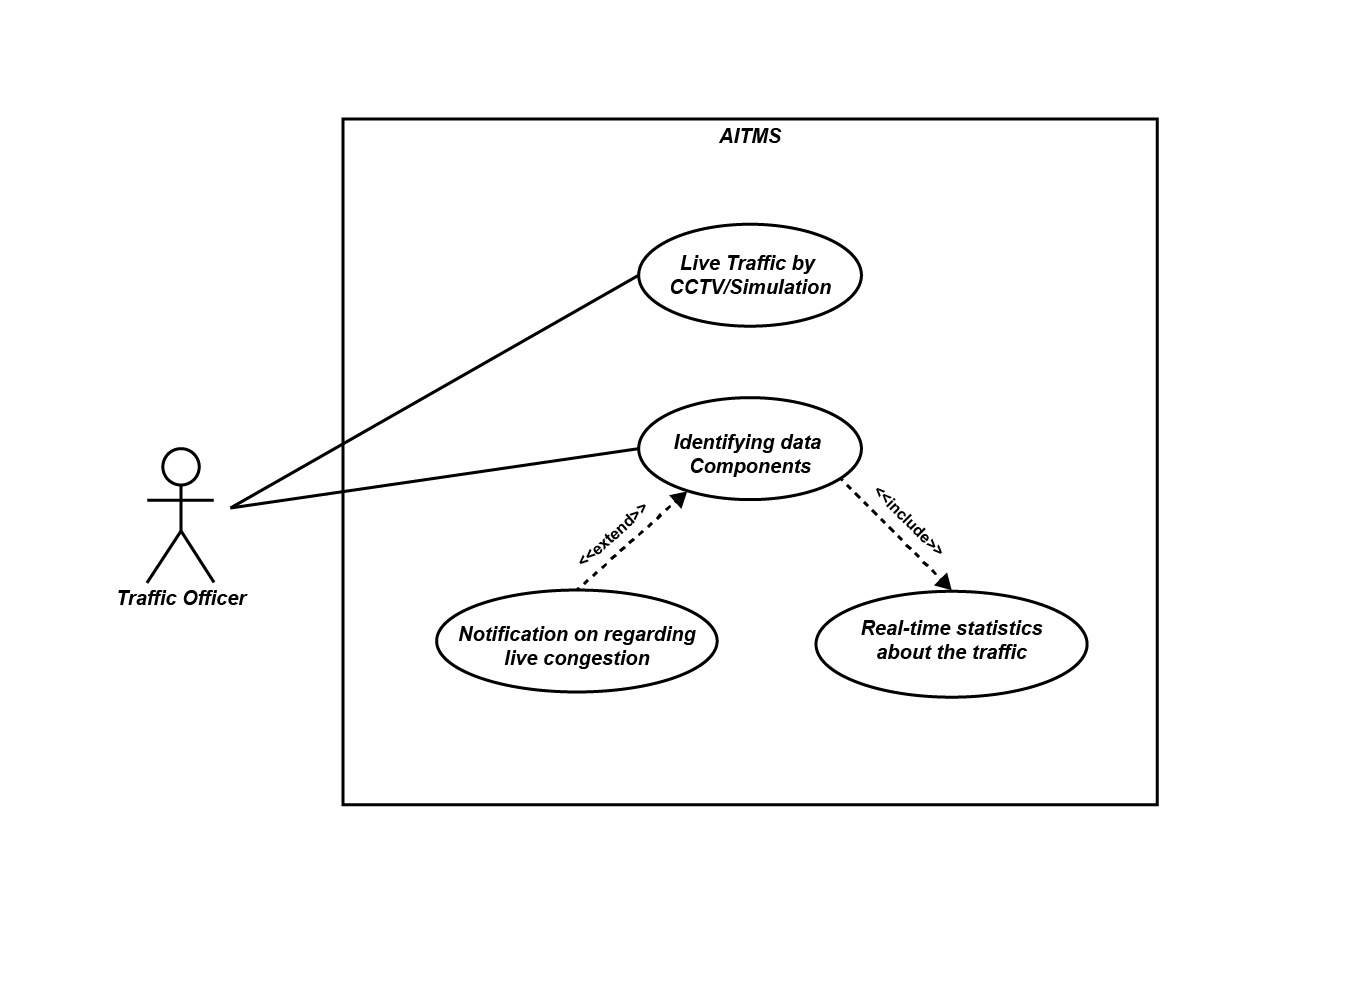
\includegraphics[height=6in]{./Diagrams/PNG/uml}
		\caption{Use Case Diagram}
	\end{figure}
	
	\begin{comment}
		\newpage
		\section{Class Diagram}
		\hspace*{0.5in}The class diagram shows the building blocks of any object oriented system. Class diagram depicts a static view of the model or part of the model, describing what attributes and behavior it has rather that the detailing the methods of achieving operations. Class diagrams are most useful in illustrating relationships between classes and interfaces. Generalizations, aggregations, and associations are all valuable in reflecting interface, composition or usage and connections receptively.\\
		\hspace*{0.5in}The Figure 6.2 illustrates aggregation relationships between classes. The lighter aggregation indicates that the class ObjectExplorer used ThumbNail, but does not necessarily contain an instance of it.The strong, composite aggregations by the other connectors indicate ownership or containment of the source classes by the target. Class, for example VideoPlayer  values will be contained in TableOfContents.
	\end{comment}
	\newpage
	\section{Activity Diagram}
	\hspace*{0.5in}Use cases show what your system should do. Activity diagrams allow you to specify how your system will accomplish its goals. Activity diagrams show high-level actions chained together to represent a process occurring in your system. An activity diagram is essentially a flowchart, showing flow of control from activity to activity. Unlike a traditional flowchart, an activity diagram shows concurrency as well as branches of control. Activity diagrams focus on the dynamic flow of a system.\\
	\begin{comment}\hspace*{0.5in}An activity is the process being modeled, such as using the M-Learning application. An action is a step in the overall activity, such as select subject, select topic. The flow of the activity is shown using arrowed lines called edges or paths. The arrowhead on an activity edge shows the direction of flow from one action to the next. A line going into a node is called as an incoming edge, and a line exiting a node is called an outgoing edge. Fork Node is used to show the parallel or concurrent actions. Fork has single incoming flows and multiple outgoing flows. The join means that all incoming actions must finish before the flow can proceed past the join. Join has multiple incoming flows and single outgoing flow.
	\end{comment}
	\begin{figure}[H]
		\centering
		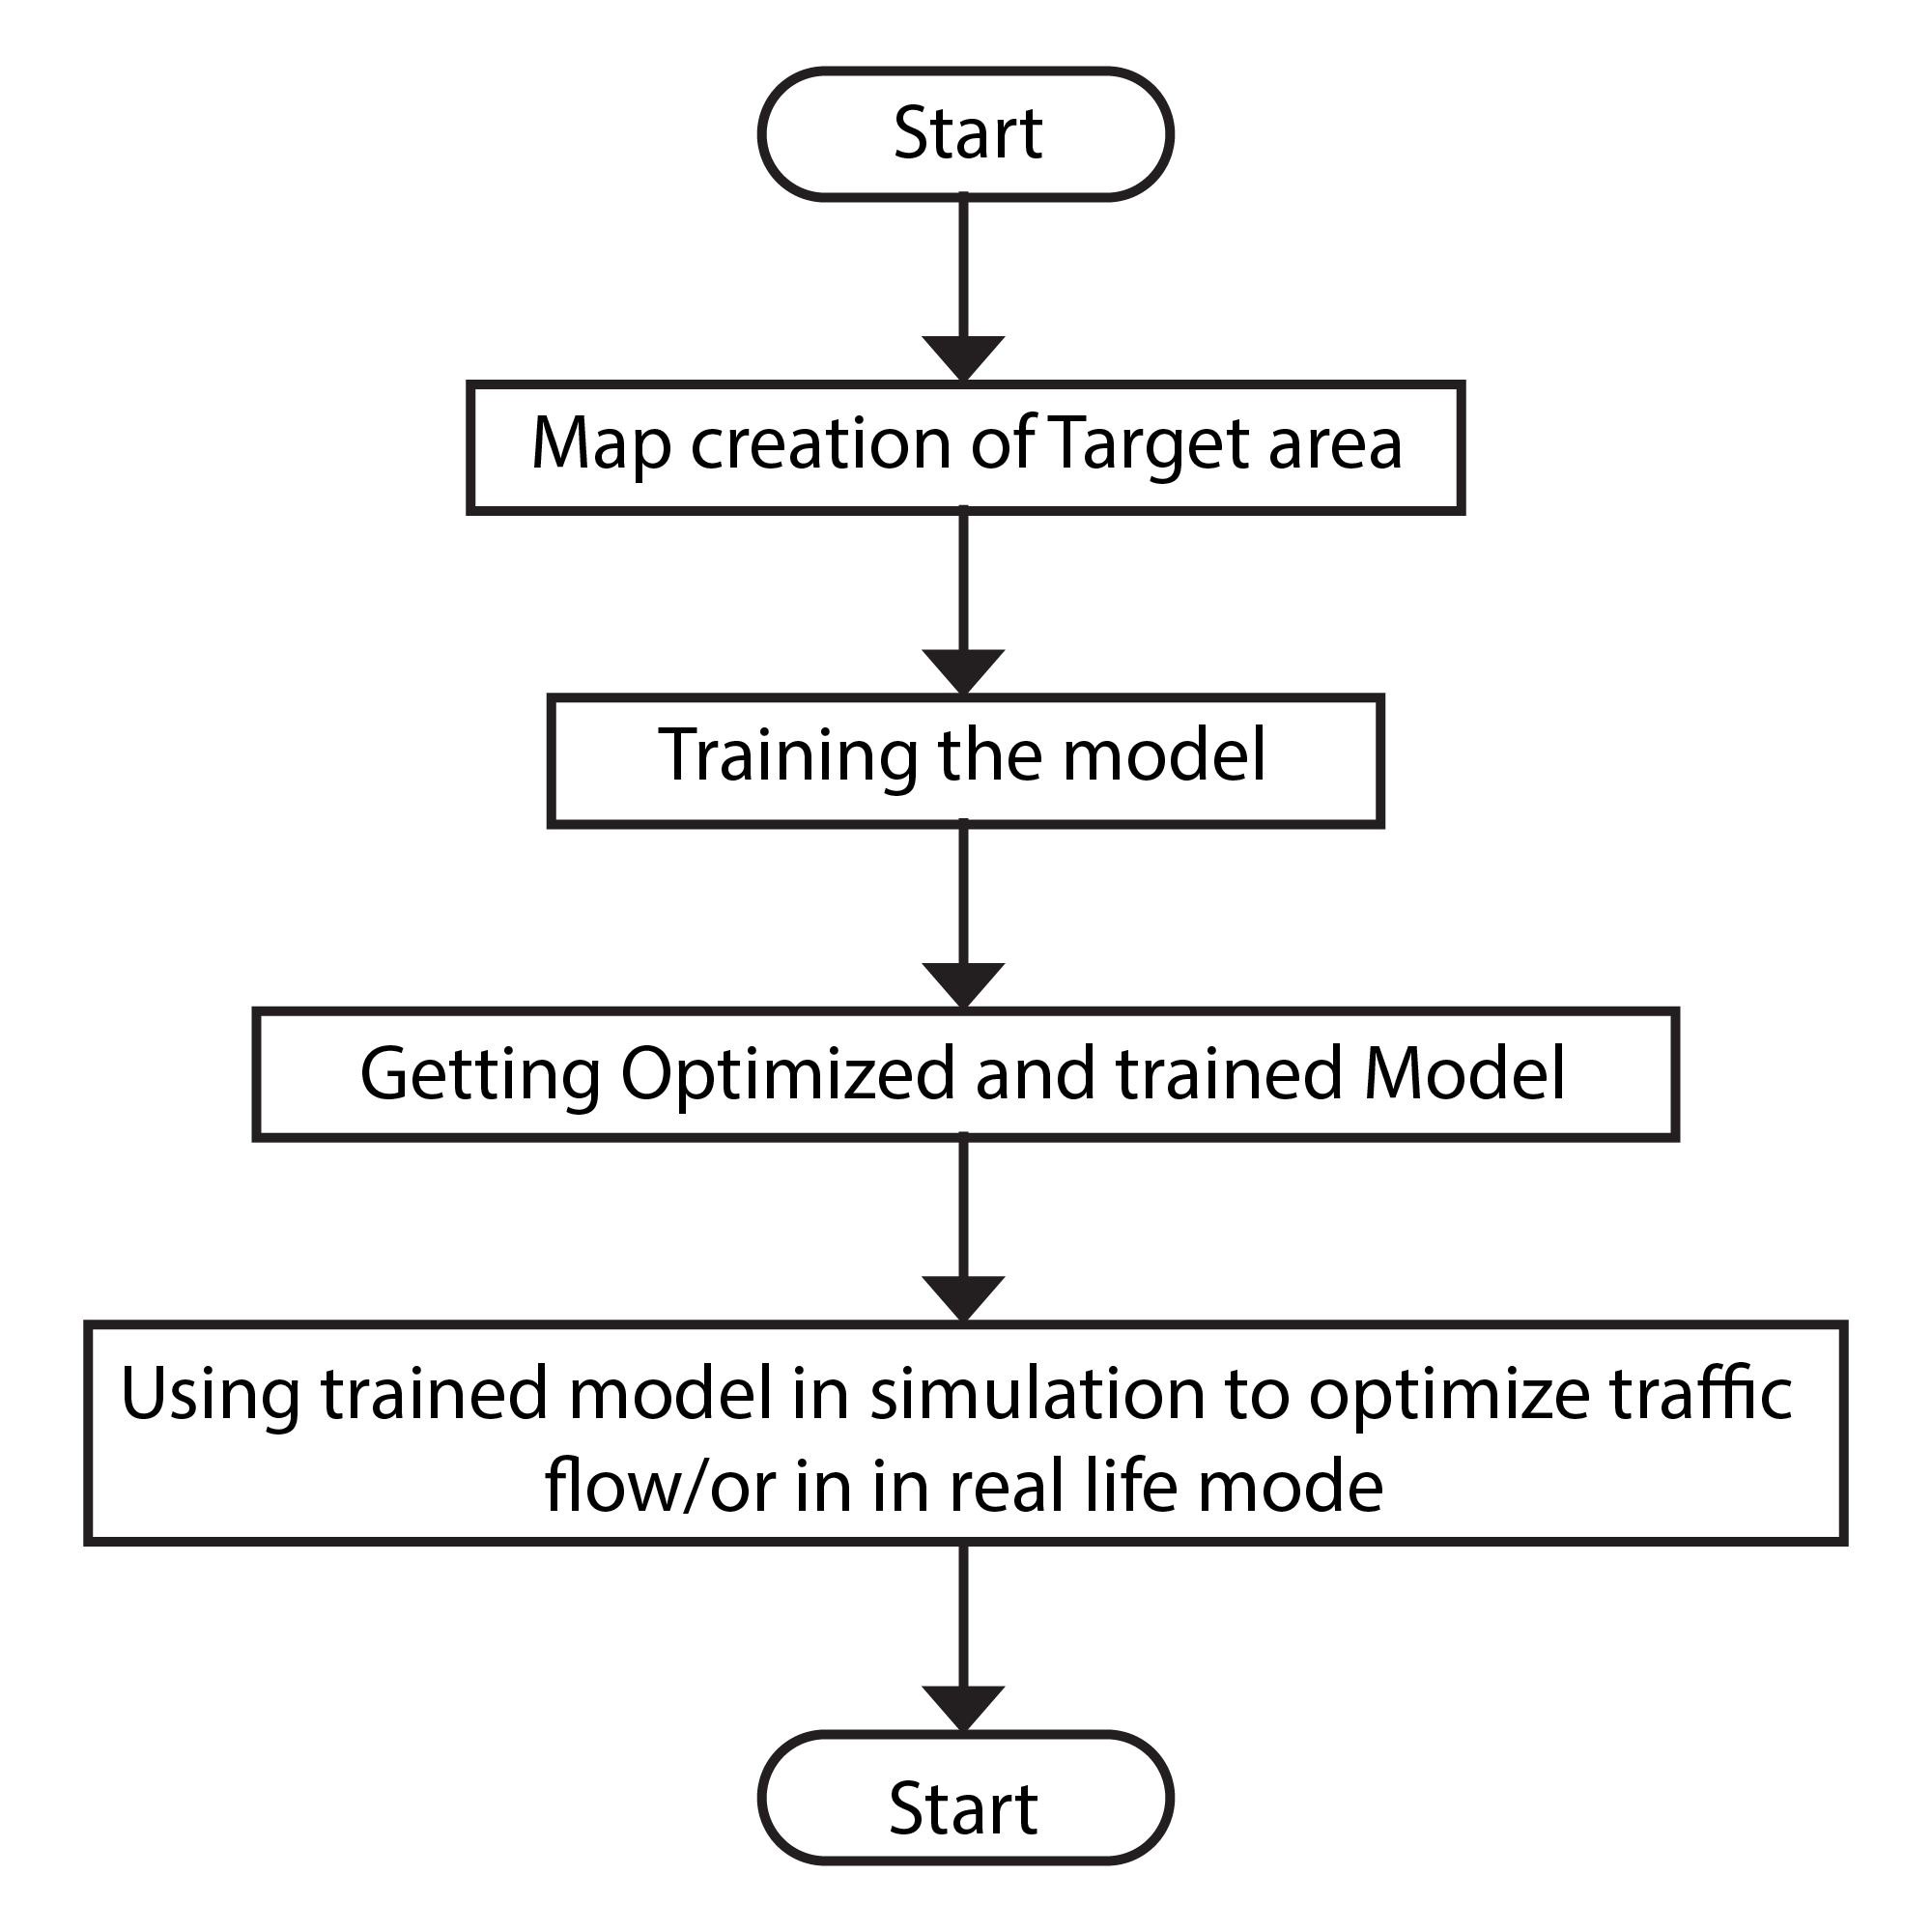
\includegraphics[width=3.2in,height=6in]{./Diagrams/PNG/flow}
		\caption{Use Case Diagram}
	\end{figure}
	\newpage
	
	\begin{comment}
		\section{Sequence Diagram}
		\hspace*{0.5in}The sequence diagram is used primarily to show the interactions between objects in the sequential order that those interactions occur. Developers typically think sequence diagrams were meant exclusively for them. However, an organization's business staff can find sequence diagrams useful to communicate how the business currently works by showing how various business objects interact.Sequence diagrams illustrate how objects interact with each other. They focus on message sequences, that is, how messages are sent and received between a number of objects. The main purpose of sequence diagram is to show the order of events between the parts of system that are involved in particular interaction.\\
		\hspace*{0.5in}The basic element of sequence diagram is collection of participants, that is, the parts of the system that interact with each other during the sequence. The participants are arranged horizontally with no two participants overlapping each other. in Figure 6.4 developer, framework, applications are some examples of participants. A message is communication between objects that conveys information with the expectation that action will be taken. An event is any point in an interaction where something occurs. Message can flow in whatever direction makes sense for the required interaction from left to right, right to left, or even back to the Message Caller itself.
		
		
		\newpage
		\section{Package Diagram}
		\hspace*{0.5in} Package diagrams are used to reflect the organizations of packages and their elements, and provide a visualization of their corresponding name space. Following are the elemts of package diagram:
		\begin{itemize}
			\item{\textbf{Package:} A package is a namespace as well as an element that can be contained in other package's namespace. A package can own or merge with other package, and its elements can be imported into a package's namespace.}
			\item{\textbf{Class:} A class is a representation of objects, that reflects their structure and behavior within the system. It is a template from which actual running instances are created. A class may have attributes and methods.}
			\item{\textbf{Interface:} An interface is a specification of behavior that implements agree to meet, it is a contract. By implementing an interface, classes are guaranteed to support a required behavior.}
			\item{\textbf{Object:} An object is an instance of a class at runtime. Objects are often used in analysis to represent the numerous artifacts and items that exist in any business.}
			\item{\textbf{Table:} A table is a stereotyped class. It is drawn with a small table icon in the upper right corner. A table element has special properties dialog with settings for database type and ability to set column information and data related operations such as triggers and indices.}
		\end{itemize}
		
		
		\newpage
		\section{State Machine Diagram}
		\hspace*{0.5in}A state machine diagram models the behavior of a single object, specifying the sequence of events that an object goes through during its lifetime in response to events. In figure 6.6, the state machine diagram shows the states the that a video or an audio file goes through during its lifetime. The file can be in one of the four states Play, Pause, Seek or Stop. It can respond to the events Play, Pause, Seek and Stop. Notice that not all events are valid in all states. For example; if a video is stopped, you cannot pause it until you play it. Also notice that a state transition can have a guard condition attached. If the file is stopped it can only respond to the play event.
		
		\newpage
		\section{Object Diagram}
		\hspace*{0.5in}In UML, an object diagram is a diagram that shows complete or partial view of the structure of a modeled system at a specific time. This snapshot focuses on some particular set of object instances and attributes and link between instances. Object diagrams are useful in understanding class diagrams. They don't show anything architecturally different to class diagram, but reflects multiplicity and roles. Basically an object diagram shows a set of objects and their relationships at a specific point in time.\\
		\hspace*{0.5in}To draw an object diagram, the first thing is to add the actual objects themselves. Object notation is actually very simple if one is familiar with class notations; an object is shown with a rectangle just like a class, but to show that this is an instance of a class rather than the class itself, the title is underlined. An object is representation of an entity. Each object in  a system has three characteristics: state, behavior and identity. The state of an object is one of the possible conditions in which it may exist, the state of an object typically changes over time.
		\newpage
		
		
		\newpage
		\section{Component Diagram}
		\hspace*{0.5in}Component diagram are one of the two kinds of diagrams found in modeling the physical aspects of object oriented systems. A component diagram shows organization and dependencies among set of components. Component diagram can be seen to model the static implementation view of a system. This involves modeling the physical things that resides on a node, such as executables, libraries, tables, files and documents.\\
		\hspace*{0.5in}Component diagram shows a set of components and their relationships. Graphically a component diagram is a collection of vertices and arcs. Component diagrams commonly contain,
		\begin{itemize}
			\item{\textbf{Components}}
			\item{\textbf{Interfaces}}
			\item{\textbf{Dependency, generalization, association and realization relationships.}}
		\end{itemize}
		
		\newpage
		\section{Deployment Diagram}
		\hspace*{0.5in}he deployment diagram depicts the runtime architecture of devices, execution environments and artifacts that reside in this architecture. It is the ultimate physical description of the system topology, describing the structure of the hardware units and the software taht executes on each unit. The deployment diagram shows how a system will be physically deployed in the hardware environment. Its purpose is to show where the different components of the system will physically run and how they will communicate with each other.
	\end{comment}
	
	\section{Summary}
	\hspace*{0.5in}Thus the various modeling techniques used for the design of Artificially Intelligent Traffic Management System were seen in this chapter.
	
	\begin{comment}
		content...
		
		%*****************************Chapter 7******************
		\chapter{Implementation and Results}
		\hspace*{0.5in}This chapter consists of the various implementation details and snapshots of the M-Learning Application developed using the Artificially Intelligent Traffic Management System.
		
		\section{Implementation Details}
		\hspace*{0.5in}This section describes the various features of the Maggie and also describes the implementation methods. Following are some of the features explained with their implementation details:\\
		\begin{itemize}
			
			\item{\textbf{Multilingual Application:}}The Multilingual feature is one of the most important features provided by the framework. The framework provides support for the Hindi language along with English; which is a primary language. The framework can provide support for more languages if required. This is implemented using the language packs of the respective language. Using the Language button on the transparent bar the user can switch between the languages. The user input is recorded in a text file and depending upon the user language selection the typeface of the content titles is changed. The content like theory animations also can be changed to respective language if recorded in that language.
			
			\item{\textbf{Social Networking Interface (SNI):}} The SNI consists of Twitter and Facebook. This implementation requires the supporting archives and libraries for both Twitter and Facebook. The Twitter and Facebook provides the app interface to facilitate the interaction and related activities. The authentication is done using these app interfaces.The library Twitter 4J is required for the Twitter SNI Support. The OAuth Authentication is used for the authentication. This requires signing up for the Twitter App which provides with the consumer key, secret key and callback url. Using this authentication is done. When the framework app user first uses the Twitter, it asks for the authorization to the Twitter App and then after the authentication the user is directed to his/her account. Then the user can publish the posts. 
			
			\item{\textbf{Logger:}}The Logger is basically used for the keep track of the usage of the framework application. It logs the activities performed by the user to a text file on the SD card. It stores information like the Device Manufacturer, Device Name, Android Operating System version, Subject being consumed and the other activities performed during learning with date and time. The Logger can also be used for error detection and correction. By tracking through the log files the reason for the failure can be uncovered.
			
			\item{\textbf{Objective Test Taking:}}The Objective Test Taking provide the user/learner to assess the knowledge consumed using the framework app. The question along with four options is displayed when the user starts the test. Out of the four options one is the answer. The user has to select one option and proceed to next question. At the end of the test the result is displayed and also the user can verify the answers. The SQLite version 3.7 is used for storing the questions and answers. By clicking on the next button the next question and associated options are retrieved.
			
			
			\item{\textbf{Interactive Objects:}}The interactive objects explorer provides the user with the various interactive objects to interact with and consume knowledge through the touch based interaction. This is implemented using the FLASH \& HTML support for mobile devices. The framework app lists the HTML interactive files stored on the SD card. The user can then select between those for learning. When a selection is made the HTML code triggers the respective SWF file and the interactive object is displayed. User can then interact using the touch and gain knowledge.
			
		\end{itemize}
		
		\section{Results}
		\hspace*{0.5in}The snapshots below are taken on the mobile device itself having Android 2.3.3 operating system, screen of 5 inches with a resolution of 800 x 480.\\
		\hspace*{0.5in}Following are the snapshots of M-Learning Application:
		
		\section{Summary}
		\hspace*{0.5in}In this chapter we discussed the implementation details of the Artificially Intelligent Traffic Management System and also the implementation of various features included in the application. We also saw the results in the form of snapshots of the M-Learning Application.
		
		%*****************************Chapter 8******************
		
		\chapter{Testing}
		\hspace*{0.5in}This chapter includes the details of Formal Technical Review meetings and describes the process carried during the review process. It also includes the Test Plan adopted for testing the Artificially Intelligent Traffic Management System and Application.
		\section{Formal Technical Review}
		\hspace*{0.5in}Formal Technical Reviews and Inspections of documents or software are performed to identify and
		remove defects. The Formal Technical Review of our project was carried at regular intervals in the form of stand-up meetings and brainstorming sessions conducted in presence of the director of Cognifront  Mr. Suchit Tiwari. The process included verification of the checklist which was developed for the review process ,the code review  checklist template is as follows:
		
		\begin{itemize}
			\item{\textbf{Does the code conform to Hungarian Notations?}}
			\item{\textbf{Is the code well-structured , consistent in style and consistently formatted?}}
			\item{\textbf{Are all variables properly defined with meaningful,consistent and clear names?}}
			\item{\textbf{Are there any redundant or unused variables?}}
			\item{\textbf{Does the code consist of comments ?}}
			\item{\textbf{Is the code error free?}}
			
		\end{itemize}
		
		\section{Test Plan}
		\begin{longtable}{|p{3.5cm}|p{5cm}|p{3.5cm}|p{1.7cm}|} \hline
			\textbf{Module being Tested}	&\textbf{Expected Result}	&\textbf{Actual Result}	&\textbf{Verdict} \\\hline\hline
			Tray Control	&When application starts, the tray should be closed. When we click on the closed tray, the tray must open up in sliding manner. And it must close, when we close the application or remove the focus from it. 	 &Tray opened successfully and closed upon removing focus. &PASS\\\hline
			Tool Tip &On a single click over a particular content a tip must appear on the screen in a fade-in and fade-out manner. &Tool Tip displayed Successfully on single clicking over the content. &PASS \\\hline
			About Cognifront &On clicking the ABOUT thumbnail the EULA, Contact and Help must be displayed. &The contents of ABOUT that are EULA,Contact and Help are shown. &PASS \\\hline
			Video Collection Page &On starting the application, video thumbnails must appear as list and the video title must be shown on the thumbnail. On clicking the video thumbnail, the video should be played. The user must be able to play,pause and stop the video. &Video Thumbnail and title displayed successfully.Video played successfully. User allowed to pause and stop the video. &PASS \\\hline
			Navigation Bar &The Navigation Bar must appear on every screen of the respective learning application. It must consist of PREVIOUS and HOME screen buttons. On Clicking the previous button, previous screen must be shown and clicking the HOME button user must be returned to home screen of the application. &Navigation Bar displayed successfully on every screen of the respective learning application. Performs returning to the previous screens and home screen successfully. &PASS \\\hline
			Objective Test Taking &When the test starts user should answer the question by selecting the appropriate option and submit it by clicking it on SUBMIT button.  On clicking the NEXT button next question must appear. To end the test user must click END TEST button and the result must be shown. &Test started successfully, questions and their options displayed properly and answer submitted successfully. Test result displayed. &PASS \\\hline
			EULA &On Clicking the EULA thumbnail the End User's License Agreement must be displayed. &EULA contents are displayed. &PASS \\\hline
			Contact &On Clicking the Contact thumbnail the Contact details of the respective authority must be displayed. &Contact details are displayed successfully. &PASS \\\hline
			Help &On Clicking the HELP thumbnail the HELP contents of the respective application must be displayed. &Help contents are displayed successfully. &PASS \\\hline
			Object Explorer &On clicking the Object Explorer thumbnail in the application menu the content as Objects must be displayed. On clicking the Object thumbnail the appropriate content must be shown. &Objects are displayed as grid of items and appropriate content is shown on clicking it.  &PASS \\\hline
			Solved Problems &On clicking the Solved Problem thumbnail the menu must be shown. The menu must consist of Printable and Animated options. &Solved Problems thumbnail displays the menu on clicking it. &PASS \\\hline
			Search &When user enters the content to be searched, the relevant results must be displayed if content is found otherwise no results should be displayed. &Search completed  successfully if required content found else no results displayed. &PASS \\\hline
			Printable &On clicking the Solved Problem thumbnail the menu must be shown. The menu must consist of Printable and Animated options. Clicking on the option Printable in the menu opens the Solutions as Thumbnail Tile List. Clicking on any particular Solution opens it and provides the printing facility. &Printable option opens and displays the Solutions as Thumbnail Tile List and Solutions open on clicking them providing the printing facility. &PASS \\\hline
			Animated &On clicking the Solved Problem thumbnail the menu must be shown. The menu must consist of Printable and Animated options. Clicking on the option Animated in the menu opens the Solutions as Thumbnail Tile List. Clicking on any particular Solution opens it and the Animation is played. &Animation option opens and displays the Solutions as Thumbnail Tile List and Solutions open on clicking it and Animation is played. &PASS \\\hline
			Audio Recorded Notes &On clicking the Record button user must be able to Record the notes in his voice and save them. &Notes recorded and Saved properly. &PASS \\\hline
			Subject Title &When user  starts the Subject Application Subject Title must be displayed. &Subject Title  displayed. &PASS \\\hline
			Thumbnail &When user starts the application, the application contents must be displayed as Thumbnails. &The  contents are displayed  as Thumbnails. &PASS \\\hline
			Title List &When user starts the application, the application contents must be displayed as Scrollable List of Thumbnails. User must be able to flick or scroll the list of thumbnails up and down. &The contents are displayed as Scrollable List of  Thumbnails. The List can be Scrolled up and down. &PASS \\\hline
			Table of Content &When user starts the application, the application contents must be displayed as Table of Contents. User must not be able to flick or scroll Table of Contents up and down if enough Contents are not present in the Table. &Table Of Contents is  displayed. The List cannot be scrolled up or down. &PASS \\\hline
			Bookmark Manager &User must be able to select the content to be bookmarked. The User must be able to Save the bookmark. &Content can be bookmarked and saved. &PASS \\\hline
			Audio Player &User must be able to play the audio by clicking on the respective content. &Audio can be played. &PASS \\\hline
			Video Player &When user starts the application, the application contents must be displayed as Scrollable List of Table of Contents. User must be able to flick or scroll the list of Table of Contents up and down. User must be able to select the Content by tapping it. The respective content must be played in the Video Player. &Table Of Contents is  displayed. The List can be scrolled up or down. The Content can be selected. The Content is played in the Video Player upon tapping it. &PASS \\\hline
			\caption{Test Plan for Artificially Intelligent Traffic Management System}
			\label{tab:nnwork}
		\end{longtable}
		
		\section{Summary}
		\hspace{0.5in}In this chapter we have described the formal technical reviews and the outcome of those. We have described the Test Plan which was successfully carried out at regular development phases.\\
		
	\end{comment}
	
	%*******************t**********Chapter 9******************
	\chapter{Technical Specifications}
	\hspace*{0.5in}In this chapter discuss the hardware and software requirements of the proposed Artificially Intelligent Traffic Management System.
	
	\begin{comment}
		
		\section{Advantages}
		\hspace*{0.5in}A key benefit of M-Learning is its potential for increasing productivity by making learning available anywhere, anytime. Because mobile devices have the power to make learning even more widely available and accessible, mobile devices are a natural extension of eLearning. M-Learning is the power of learning that is truly “just-in-time” where you could actually access training at the precise place and time on the job that you need. Our project provides the reusable piece of code that will help the developers for developing multiple M-Learning applications easily; one can also prepare audio or textual notes on move. The greatest benefit of this delivery is the combination of true interactivity coupled with portability.
		\\Following are some more advantages of Artificially Intelligent Traffic Management System:
		\begin{itemize}
			\item{\textbf{Just in time learning:}Learning at the point of need.}
			\item{\textbf{Ability to access learning (almost) everywhere:}This means down time can be leveraged for learning.}
			\item{\textbf{Potential to be two way and multi-media:}Video, powerpoint, podcasts, and quizes are all potential outputs to iPhone devices. This provides a great deal of flexibility for mobile development.}
			\item{\textbf{Potential for location based learning:}This means the phone can alert the person when they are near a potential learning experience based in the context in which the learning will be used–which potentially can help retention and return on investment.}
		\end{itemize}
		
		\section{Limitations}
		\hspace*{0.5in}To participate in mobile learning one must have a tablet or mobile devices with android as its base operating system,these can have high ranges of cost, due to this reason it cannot be affordable by everybody in todays world.
		\\
		\hspace*{0.5in}Another aspect to be considered is the size of the device, this is only a challenge if one incorrectly plans mobile learning content to be nothing more than compressed eLearning. If your users are already using their mobile device that you plan to push learning to, your strategy should be what content do they need in the context of using the device. Add to that, the greatly improved displays, such as the OLED display on the DROID Incredible, and size isn't a detriment any more, but an advantage.
		
		\section{Applications}
		\hspace*{0.5in}The Artificially Intelligent Traffic Management System can be used in following areas:
		\begin{itemize}
			\item{Institutions for teaching the learning material developed by the developer for mobile learning.}
			\item{Students can study with ease.}
			\item{The education application developer can use this framework for developing number of applications that can be imported on mobile devices.}
		\end{itemize}
		
	\end{comment}
	\subsection{Hardware Requirements}
	\begin{itemize}
		\item{Intel Core i5 8300H or equivalent/higher}
		\item{16GB RAM for application development}
		\item{Min. 16 GB Space in Hard Disk}
	\end{itemize}
	
	\subsection{Software Requirements}
	\begin{itemize}
		\item{Visual Studio 2019}
		\item{Unity 2020.3}
		\item{Python 3.7 or higher}
		\item{YOLO 3.0 or higher}
		\item{TensorFlow 2.0 or higher}
		\item{GIMP and Photoshop}
	\end{itemize}
	
	\section{Summary}
	\hspace*{0.5in}This chapter discusses the various hardware and software requirements of the project.
	%***************************Chapter 10**************
	\chapter {Future Scope}
	
	\hspace{0.5in}Scalability is an essential feature for traffic management systems in current age. As the number of vehicles and roads increases for a particular locality, it's traffic management system must be able to handle the changes in maps and traffic flow. Keeping this in mind, the proposed system provides the following future possibilities:\\
	
	\begin{itemize}
		\item{Warehousing of parametric data and reports to analyze periodic patterns and improve optimization using data collected over use. This gives the opportunity to use data science concepts to improve existing traffic management systems and even other roadway infrastructure.}
		\item{The ability to connect multiple AITMS will greatly improve scalabbility and optimization. If nieghboring solutions can work together, providing an additional layer of optimization using their combined data becomes possible.}
		\item{Improving on library of optimization algorithms. Since, different algorithms may suit different maps, having a variety of algorithms in the toolkit becomes helpful.}
		\item{Integration of additional functionalities such as incident detection, manual control, etc.}
	\end{itemize}
	
	%*****************************Chapter 11**********
	\chapter{Conclusion}
	\hspace*{0.5in}The proposed system will be able to minimize congestion and will be able to report various statistics regarding congestion and traffic incidents in real time. The system also provides sufficient scope for scalability and additional functionalities which will help cope with rising number of vehicles and roads. 
	Furthermore, the aim of the project in the coming phases will be to perform simulations of various optimization algorithms in order to validate the system for real life implementation.
	
	\begin{comment}
		
		%**************************Appendix******************
		
		\appendix
		\cleardoublepage
		\addtocontents{toc}{\bigskip}
		\addcontentsline{toc}{part}{Appendix}
		
		\chapter{Glossary}
		\begin{itemize}
			\item{\textbf{Maggie:}} We have code named our project Artificially Intelligent Traffic Management System as Maggie.
			\item{\textbf{M-Learning:}} The application of small, portable, and wireless computing and communication devices like Laptops with Wireless LAN technology, mobile phones, Personal Digital Assistants (PDAs) with Bluetooth or IRDA interfaces for communication and computing.
			\item{\textbf {TOC:}} The term stands for Table of Contents which is a collection of contents. It can be used by the user to view the collection of learning materials available in the application.
			\item{\textbf {OEM:}} The term stands for Original Equipment Manufacturer, it is used to generate a logo for a particular application. Once an OEM logo is generated all the responsibilities are upto the manufacturer i.e. if any problem arises the manufacturer has to look after it till the problem is solved.
		\end{itemize}
		
		\chapter{Achievements}
		\begin{itemize}
			\item{\textbf{First prize at CSI's National Level Discover Thinking}\\
				\hspace*{0.5in}We had participated in \textbf{Computer Society of India's (CSI)} National Level Project Competition Discover Thinking sponsored by \textbf{Microsoft}. The contest had 3 rounds, 1st round at CSI chapter level held at particular colleges, 2nd round at CSI regional level held at Pune, and final round was at national level held at Coimbatore, Tamilnadu. Among 90 projects across the country our project was ranked at the first place after rigorous evaluation conducted by an eminent panel of judges from industry and educational background. }
			\item{\textbf{Published Research Paper in IJSER 2012}\\
				\hspace*{0.5in}We have published a research paper titled \textbf{Artificially Intelligent Traffic Management System} in \textbf{International Journal of Scientific and Engineering Research (IJSER)}. Our paper is published in the May edition of IJSER 2012.}
		\end{itemize}
		\vspace{5in}
		content...
		
		\newpage
		\addcontentsline{toc}{chapter}{Bibliography}
		
	\end{comment}
	
	\begin{thebibliography}{99}
		
		\bibitem{paper1}\emph{You Only Look Once: Unified, Real-Time Object Detection}; Joseph Redmon, Santosh Divvala, Ross Girshick and Ali Farhadi, 2016.
		
		\bibitem{paper2}\emph{Traffic Congestion Detection from Camera Images using Deep Convolution Neural Networks}; Pranamesh Chakraborty, Yaw Okyere, Subhadipto Poddar, Vesal Ahsani, Anuj Sharma and Soumik Sarkar. In Transportation Research Record Journal of the Transportation Research Board, June 2018. DOI: 10.1177/0361198118777631
		
		\bibitem{paper3}\emph{Smart Control of Traffic Light Using Artificial Intelligence}; M. M. Gandhi, D. S. Solanki, R. S. Daptardar and N. S. Baloorkar. 2020 5th IEEE International Conference on Recent Advances and Innovations in Engineering (ICRAIE), 2020, pp. 1-6, doi: 10.1109/ICRAIE51050.2020.9358334.
		
		\bibitem{paper4}\emph{Comparison of Current Practical Adaptive Traffic Control Systems.}; Hongyun Chen \& Jian Lu. (2010). 1611-1619. 10.1061/41127(382)176. 
		
		
		%\url{Your url of reference}
	\end{thebibliography}
\end{document}